\documentclass{sig-alternate}
\usepackage[utf8]{inputenc}
\usepackage[T1]{fontenc}

\newcommand{\superscript}[1]{\ensuremath{^{\textrm{#1}}}}
\def\sharedaffiliation{\end{tabular}\newline\begin{tabular}{c}}
\def\wu{\superscript{*}}
\def\wg{\superscript{\dag}}

\usepackage{listings} 

% Typography
\usepackage{times}
\usepackage{mathptmx}
\usepackage{microtype}
\usepackage[normalem]{ulem}
\usepackage[pdftex,bookmarks,bookmarksopen,bookmarksdepth=2,
            urlcolor=black,colorlinks=true,linkcolor=black,citecolor=black]{hyperref}
\usepackage[capitalize,noabbrev]{cleveref}
\def\UrlFont{\em}

% Graphics
\usepackage{tikz}
\usepackage{tkz-graph}
\usetikzlibrary{arrows,positioning,shapes.misc}
%\let\subcaption\relax
\usepackage{graphicx}
%\usepackage[caption=false]{subfig}
%\usepackage{caption}
\usepackage{subcaption}
\captionsetup[figure]{labelfont=bf,textfont=bf}
\captionsetup[subfigure]{labelfont=normalfont,textfont=normalfont}
\definecolor{lightgrey}{RGB}{170, 170, 170}
\definecolor{darkblue}{RGB}{0, 0, 0}
\definecolor{darkred}{RGB}{170, 0, 0}
\definecolor{darkgreen}{RGB}{0, 110, 0}

% Acronyms
\usepackage{xspace}
\newcommand{\sparql}{{SPARQL}\xspace}
\newcommand{\sparqlo}{{SPARQL 1.1}\xspace}
\newcommand{\arq}{{ARQ}\xspace}
\newcommand{\wthreec}{{W\oldstylenums 3C}\xspace}
\newcommand{\sfive}{{S\oldstylenums 5}\xspace}
\newcommand{\select}{{SELECT}\xspace}
\newcommand{\construct}{{CONSTRUCT}\xspace}
\newcommand{\ask}{{ASK}\xspace}
\newcommand{\describe}{{DESCRIBE}\xspace}
\newcommand{\from}{{FROM}\xspace}
\newcommand{\odbc}{{odbc}\xspace}

% Tight lists
\usepackage{enumitem}
\setlist{nolistsep}

% Listings and Verbatim environment
\usepackage{fancyvrb}
\usepackage{relsize}
\usepackage{listings}
\usepackage{verbatim}
\newcommand{\smalllistingsize}{\fontsize{8pt}{9.5pt}}
\newcommand{\inlinelistingsize}{\fontsize{8.5pt}{11pt}}
\newcommand{\defaultlistingsize}{\inlinelistingsize}
\RecustomVerbatimCommand{\Verb}{Verb}{fontsize=\inlinelistingsize}
\RecustomVerbatimEnvironment{Verbatim}{Verbatim}{fontsize=\inlinelistingsize}
\lstset{frame=lines,captionpos=b,numberbychapter=false,escapechar=§,
        belowskip=1em,
        xleftmargin=2ex,
        framexleftmargin=2ex,
        basicstyle=\ttfamily\smalllistingsize\selectfont}
\crefname{lstlisting}{Listing}{Listings}
\definecolor{grey}{RGB}{130,130,130}

\usepackage{color}
\newcommand{\todo}[1]{\noindent\textcolor{red}{{\bf \{TODO}: #1{\bf \}}}}
\newcommand{\rv}[1]{\noindent\textcolor{red}{{\bf \{RV}: #1{\bf \}}}}
\newdef{definition}{Definition}

\begin{document}

\title{What public transit API logs tell us about travel flows}
\numberofauthors{6}
\author{
\alignauthor
Pieter Colpaert\\
\affaddr{\email{\texttt{pieter.colpaert@ugent.be}}}
\and
\alignauthor
Alvin Chua\\
\affaddr{\email{\texttt{alvin.chua@asro.kuleuven.be}}}
\and
\alignauthor
Ruben Verborgh\\
\affaddr{\email{\texttt{ruben.verborgh@ugent.be}}}
\and
\alignauthor
Erik Mannens\\
\affaddr{\email{\texttt{erik.mannens@ugent.be}}}
\and
\alignauthor
Rik Van de Walle\\
\affaddr{\email{\texttt{rik.vandewalle@ugent.be}}}
\and
\alignauthor
Andrew Vande Moere\\
\affaddr{\email{\texttt{andrew.vandemoere\\@asro.kuleuven.be}}}\\
}

\maketitle
\begin{abstract}

%Public transit schedules are made available on the Web in various ways, such as in a GTFS file, a route planning API, or through Linked Connections.
%This webservice provides an answer to a route planning question with parameters such as ``departuretime'', ``from'' and ``to''.
% Context & % Need
In the field of urban planning, researchers need an indication of how people move between cities. 
Yet, getting statistics of travel flows within public transit systems has proven to be troublesome.
% Task
In order to get an indication of travel flows between cities in Belgium,
we analyzed the query logs of the iRail API, a highly expressive route planning API for the Belgian railways.
We were able to study $\sim$100k to 500k requests for each month between October 2012 and November 2015, which is between $0.56\%$ and $1.66\%$ of the amount of monthly passengers.
% Object & Findings
Using data visualizations, we illustrate the commuting patterns in Belgium and confirm that Brussels, the capital, acts as a central hub. 
The Flemish region appears to be polycentric, while in the Walloon region, everything converges on Brussels.
The findings correspond to the real travel demand, according to experts of the passenger federation Trein Tram Bus.
% Conclusion
We conclude that query logs of route planners are of high importance in getting an indication of travel flows.
% Perspectives
However, better travel intentions would be acquirable using dedicated HTTP POST requests.
%%Redundant according to RV:
%Highly expressive transport data publishing methods such as route planning API exist, as well as data dumps or data fragments.
%In order to be able to gather meaningful logs in all cases, we suggest using a separate POST request containing the entire query.

\end{abstract}

\vspace{1em}

\section{Introduction}
\label{sec:introduction}

Today, the Belgian railway company (SNCB) takes manual samples of people getting on and off trains in stations. 
To date, this is still the SNCB's only source to determine people flows through their network\footnote{\url{http://www.belgianrail.be/nl/corporate/in-de-kijker/comptages_voyageurs_2014.aspx}}.
Also within other transit systems the data is tedious to get, certainly when passengers do not have to check-in and check-out.
Nonetheless, indications of how people move within a transit network is of uttermost importance for, amongst others, making demand-driven policy decisions concerning mobility.

The \emph{iRail} project\footnote{\url{https://hello.irail.be}} started in 2008 to make the data of the Belgian railway accessible for developers.
The project offers developers both a data dump for third party apps (since $\sim$~August~2015) and a route planning API (since $\sim$~October~2010).
The query logs of the latter has been stored since November 2012 (requests before that period got lost due to server migrations).

Getting indications of people flows through public transit networks is a challenge. 
Yet, \emph{can we not get an indication of these transit flows by studying the query logs of Web-services?}

In this paper, we give a small overview of related work to gather data for flow analysis.
Next, we introduce the iRail query logs, which we study by the means of visualizations.
Finally, we look at how public transit data is published and how we would be able to get a better indication of travel flows.

\section{Related work}
\label{sec:relwork}
%\subsection{Flow analysis}

\emph{Flow analysis} is a topic of theoretical interest and practical importance conventionally conducted to study spatial dynamics and identify routine patterns in the movement of people.
For instance, interest in modelling traffic flows emerged from the strain placed on urban transportation systems during peak hours~\cite{roth,ferreira}.
Likewise, insight into routine travel patterns is crucial for the conceptualization of functional urban areas~\cite{servillo2013town}, urban hierarchies~\cite{christaller1966central} and other territorial structures.

Over the past decade, large datasets have become increasingly commonplace due to the proliferation of sensor networks and portable devices like smartphones.
Termed ``Big Data'' due to the large volume of data records that emerge from real-time sensing~\cite{kitchin}, such datasets typically contain information of activities or processes linked to the space and time where they occur.
In the domain of ``Smart City'' research, much has been accomplished with the use of ``Big Data'' to monitor human movement.
Smart card data from public transport systems~\cite{roth,beecham}, taxi journeys~\cite{ferreira} as well as cellular call data~\cite{sevtsuk} have provided planners with new opportunities to develop greater understanding of mobility patterns in urban environments~\cite{batty}.
Yet query logs were, to our knowledge, never used for flow analysis so far.

\subsection{Studying Query Logs}

On highly expressive servers, such as \sparql-endpoints, query logs can play an important role in fine-tuning the underlying datastores~\cite{arias2011empirical}.
E.g., they determined that in 2011 in the context of the graph query language \sparql, most of the queries are simple and include few triple patterns and joins.
Furthermore, the graph patterns are usually star-shaped and despite triple pattern chains exist, they are generally short.
Other, more cacheable interfaces more to the left on the Linked~Data~Fragments axis~\cite{ldf}, also benefit from query logs in order to e.g., know who is using what clients to query the Web, yet the user intention is lost~\cite{usewod2015}.
This was called ``a blessing for privacy'', yet adding the user query as an HTTP header was suggested.

\subsection{Visualizing Travel Flows}

%Visualizations are crucial for understanding the patterns in data and representing transit flows.
Visualizations are crucial for making data analysis tangible \cite{thomas2006visual}, so that results can be communicated and debated \cite{robinson2008collaborative}. 
This is key for our research, since the questions presented are exploratory in nature \cite{kraak2008exploratory} and can be addressed in many ways. 
Movement data has received substantial attention from the visualization community and a range of techniques has been developed to support flow analysis \cite{andrienko2012visual}. 
Visualizations of flows can be broadly categorized into two groups. 
Representations that display the complete trajectory and Origin Destination (OD) type representations that take only the start and end locations into account.
Since our data solely consists of OD information, we narrow our description to the latter group of visualization techniques.

OD type representations are employed when the origin and destination preside over intermediate locations on the path of movement. The OD Matrix is the most common visualization technique based on this type of representation. 
Rows and columns correspond to locations while cells are coloured to express the volume of flow.
OD matrices can be reordered to emphasise connectivity between locations.
While this feature is particularly useful for identifying trends and outliers in the data, the tabular display is challenging for lay users to interpret and less expressive of connections between locations than representations based on the node-link metaphor \cite{holten2011extended}.
In recent years, such representations have become increasingly prominent for displaying movement in science as well as popular culture.
Locations are depicted as nodes and arrows are drawn between them to indicate movement in a certain direction, allowing for exact and individual relationships to be traced. 
This representation is detailed and straightforward to understand but becomes cluttered when multiple lines intersect. 

A number of solutions have been proposed for clutter reduction. 
Filtering is the most commonly practiced. 
The same goal can be achieved by clustering lines that have similar properties like common start, end or intermediate locations \cite{andrienko2007visual}. 
Both solutions are effective at reducing clutter yet it should be noted that excessive aggregation or filtering removes a significant amount of information from the visualization.

Another solution is to transform the visual representation. 
Flow maps \cite{phan2005flow} reduces clutter by rerouting the arrows to minimize intersection and obtain layouts that align with key geographic features like roads, rivers or coastlines. 
However, a certain degree of ambiguity is introduced to the visualization since the arrows do not depict actual paths of movement and maybe misleading to interpret.
A computationally cost effective alternative is to draw links as arcs instead of arrows \cite{chua2014flowsampler}.
Yet, this visual encoding may intensify the visual complexity of the representation.

Non-geographic representation is a viable alternative to this challenge in this specific context of visualizing flows on the rail network since the locations of stations and the exact routes between them are known and have been pre-determined. 
Thus the analytical focus and goal of visualization is to depict differences in the volume of flows between different stations. 
While many visualization techniques fulfil this purpose, we find chord diagrams \cite{krzywinski2009circos} particularly appropriate for delivering information in a compact form, allowing for comparison across multiple plots in a single view.
A further description of chord diagrams is provided in \cref{sec:vis}.

\section{The query logs}
\label{sec:logs}

The iRail API is an XML/JSON HTTP API: each request on \url{http://api.irail.be} returns a response that can be used directly in an end-user app.
It exposes four features: 
\begin{enumerate}
\item \emph{Route Planning} (\url{http://api.irail.be/connections/{?from,to,date,time}}) plans a route from one station to another, taking into account a preferred start time.
\item \emph{Next Departures} (\url{http://api.irail.be/liveboard/{?station,date,time}}) shows the next train departures in a certain station, useful for creating quick overviews.
\item \emph{Trip Status} (\url{http://api.irail.be/vehicle/{?id,date}}) returns the stations this train passes by on the day of the request.
\item \emph{List of all stations} (\url{http://api.irail.be/stations/}) gives an overview of all stations Belgian trains can arrive at.
\end{enumerate}

%IRail is a not for profit organization that stimulates digital creativity concerning mobility.
This interface is open source and we were able to suggest changes to the system in which the query logs become open data\footnote{\url{https://github.com/iRail/iRail/pull/138}}.
As of the 17th of December 2015, iRail publishes the most recent 1,000 requests done on the API as open data, each second, at \url{http://api.irail.be/logs/}.
In order to publish this data, we chose a newline-based format: each new line contains a new query object encoded in JSON. 
The JSON objects can be read one per one, so UNIX commands such as \emph{grep} work well with this format.
We chose this over CSV as we have more flexibility towards changing the object properties in the future.
Next, we chose to add an HTTP header with a link to the query log context according to the JSON-LD specification\footnote{\url{http://www.w3.org/TR/json-ld/}} to turn it into Linked Data.
%This is the JSON-LD context of all the objects in the, JSON-stream. Subsequentially, we call this a \emph{JSONLD-stream} and this has been formalized at \emph{https://github.com/pietercolpaert/jsonld-stream}.

Using this data, everyone can build their own historic query log dataset.
The server costs for iRail to host this dataset stay limited.
Furthermore, this way of publishing data enables research for real-time predictions of travel intentions.
Privacy preservation is paramount~\cite{silvestri} when dealing with query logs and, therefore, IP addresses have been removed to protect the privacy of our users. 
Additionally, the integrity of this dataset, without IP addresses, has been vetted by the Belgian Privacy Commission and permission has been granted for these query logs to be published as open data.

We are particularly interested in studying the potential application of \emph{route planning} queries as an information resource for flow analysis due to the input it captures from human users.
The other features are less relevant for this purpose as they are generally polled by digital signage providers or status boards, and thus do not reflect direct human demands.
The dataset described in this paper is compiled from the \emph{Apache} \emph{access.log} files generated between October 2012 and December 2015, filtered by ``connections'' entries.
We made a copy of this dataset available in CSV format can be downloaded at \url{https://github.com/pietercolpaert/irail-route-planning-query-logs}.
%CSV header of the final logs: datetime,requested_datetime,from_id,from_name,from_long,from_lat,to_id,to_name,to_long,to_lat,user_agent,operating_system,is_bot
Each row within this dataset contains:
\begin{enumerate}
\item A timestamp of when the request was executed,
\item The request path between two stations and their associated geographic coordinates,
\item The user-agent string cfr. RFC2616,
\item The operating system of the user-agent and
\item A flag stating if the user-agent is a bot.
\end{enumerate}

\begin{figure}
\centering
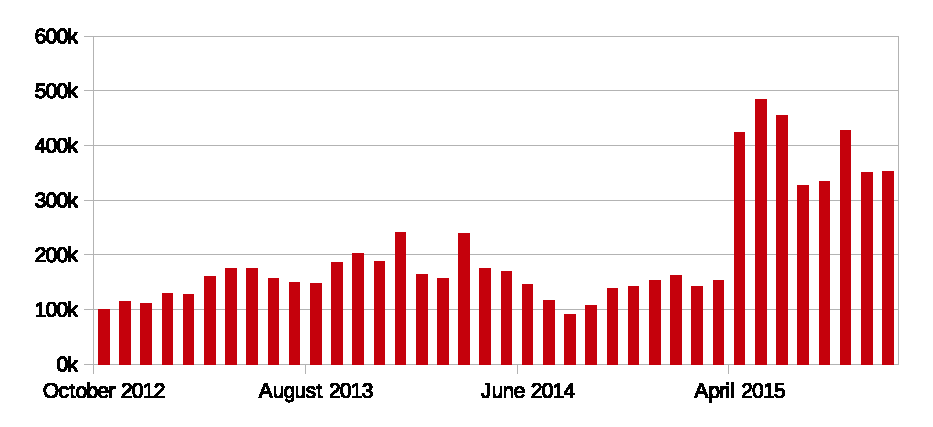
\includegraphics[width=8.6cm]{querylogs}
\caption{Amount of queries on the route planning part of the iRail API between October 2012 and December 2015. In April 2015 an official app of the Belgian railways was discontinued, which explains the sudden raise of iRail API queries.}
\label{fig:querylogs}
\end{figure}

There has been an increase in the number of queries made between 2012 and 2015. 
\cref{fig:querylogs} provides a break down of the numbers on a monthly basis. 
A distinctive increase in the number of queries can be observed in April 2015 when the official route planning service provided by of the Belgian rail company was discontinued\footnote{\url{https://hello.irail.be/2015/04/22/april-updates/}}, resulting in widespread adoption of alternative software applications built on top of the iRail API.
Calculated with indicators provided by the Flemish regional government of Belgium\footnote{\url{http://www4.vlaanderen.be/sites/svr/Cijfers/Exceltabellen/mobiliteit/vervoersprestaties/personenvervoer/MOBIOPEN006.xls}}, we infer a monthly average of 19.3, 19.4, 19,6 and 19.7 million passengers in 2012, 2013, 2014 and 2015 respectively. 
Correspondingly, the average number of iRail queries per month amounts to 0.11, 0.17, 0.15 and 0.33 million respectively.
Assuming that each request reciprocates with an intention to travel by rail, our data captures a respective $0.56\%$, 0.88\%, 0.77\% and 1.66\% of the actual journeys that have occurred.

%After analysis, it appeared 10\% of the request where performed by Google bots.

\section{Method}
\label{sec:method}

Flow analysis involves the comparison of aggregated movement between distinct locations within a specific time frame. 
In most cases, the analytical objective is to identify trends that occur in journeys made between pairs of locations and allow for the sensitivities to be explored. 
Data visualization is typically employed to facilitate in this process thus the input data must be transformed into a format that allows for the quantity and directional flow of movement to be visually encoded.
The data must undergo several stages of data processing to arrive at this outcome.

\subsection{Data Processing}

We were specifically interested in understanding how travel during the morning rush hour on weekdays differ from weekends. In this regard, the dataset was filtered to exclude data records created beyond the time range of 06:00 hours and 10:00 hours.
Queries made by automated user-agents like search engine bots and data harvesters can be considered as valid traffic but may over represent connections between certain stations.
Accordingly, such queries were excluded since they do not explicitly represent human travel behavior.
Station names tend to contain be highly inconsistent since any text information can be parsed to the API.
This may include invalid character encoding, spelling mistakes and the use of unstandardized abbreviations.
We employed an open-source reconciliator (\url{https://github.com/irail/stations}) to reduce spelling variations and remove data records with missing information. 
Through this process, station names were also linked to their corresponding geographical coordinates.

\begin{figure*}
  \centering
  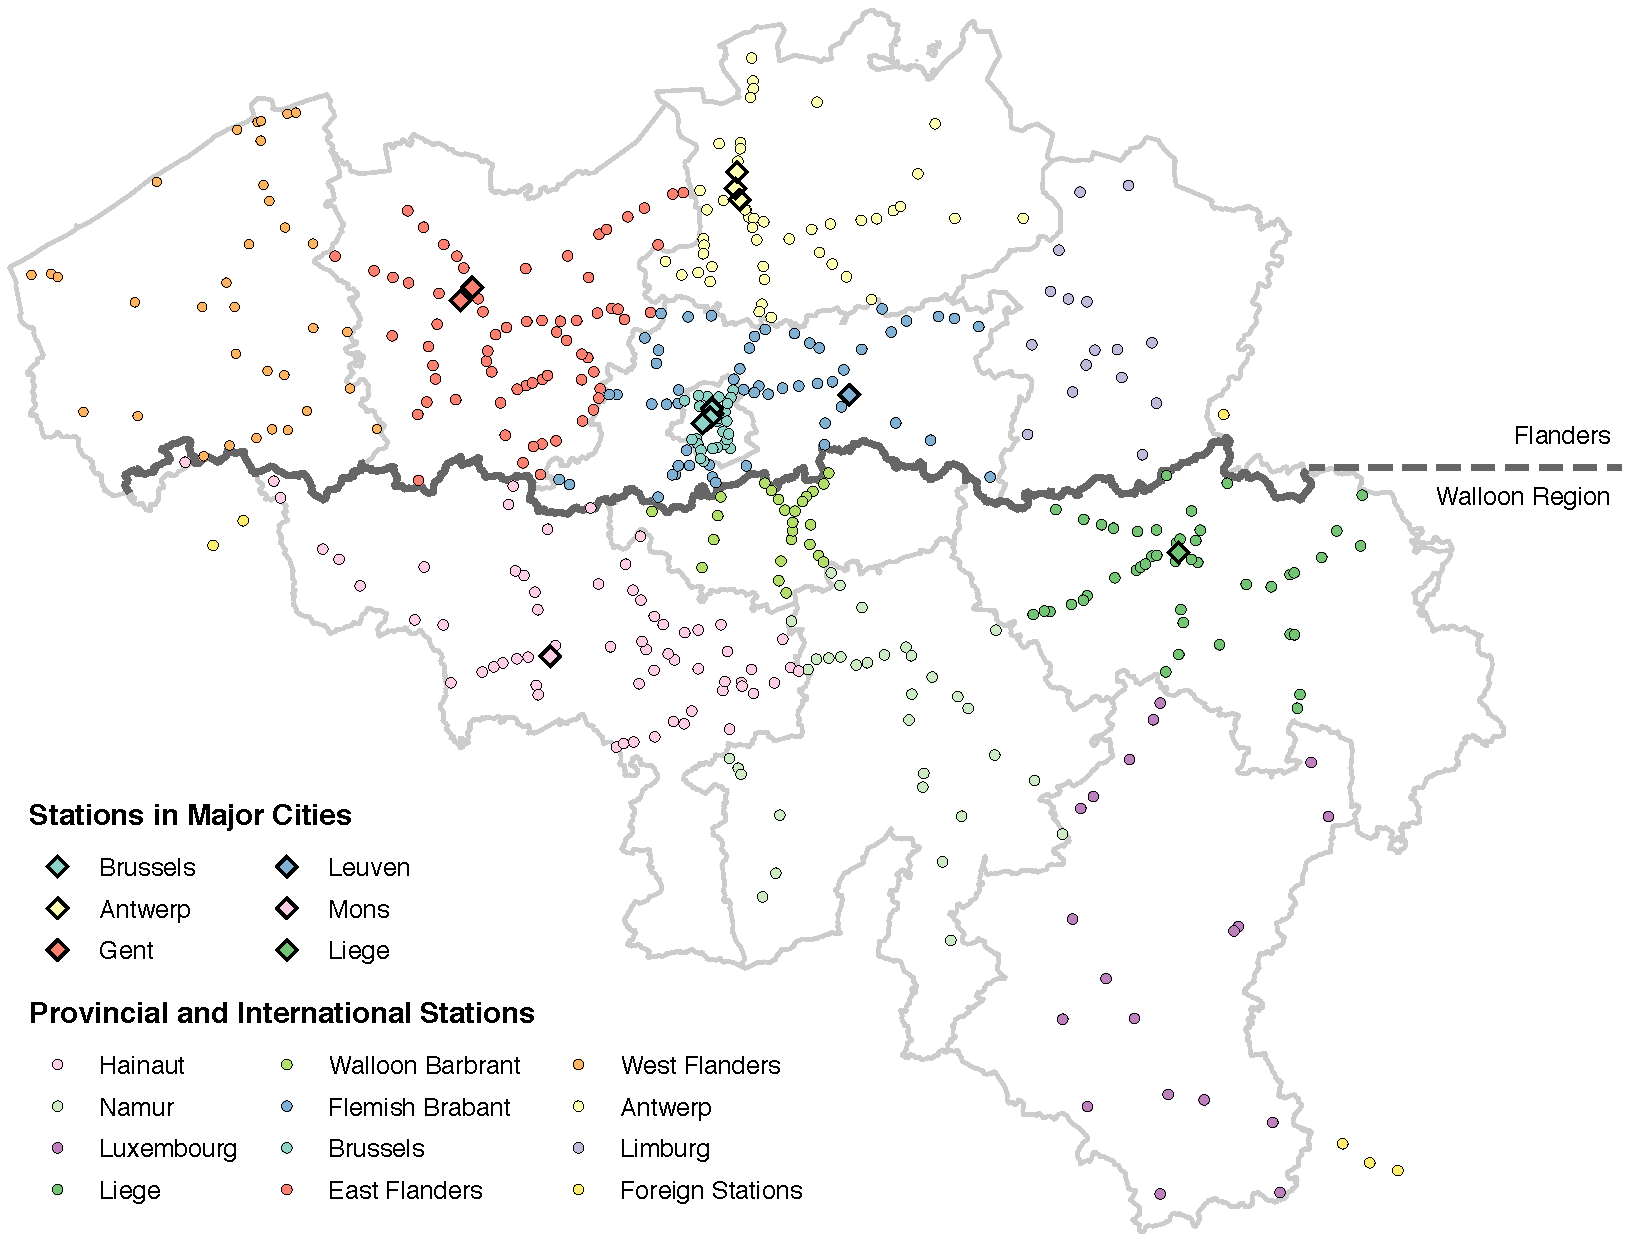
\includegraphics[width=14cm]{method-c.pdf}\\
  \caption{Each station is color coded to indicate the province it will be aggregated to. Stations in major cities as well as stations outside of Belgium are aggregated to seperate groups.}
  \label{fig:method-c}
\end{figure*}

\begin{figure}[h]
  \centering
  \begin{subfigure}{.2375\textwidth}
    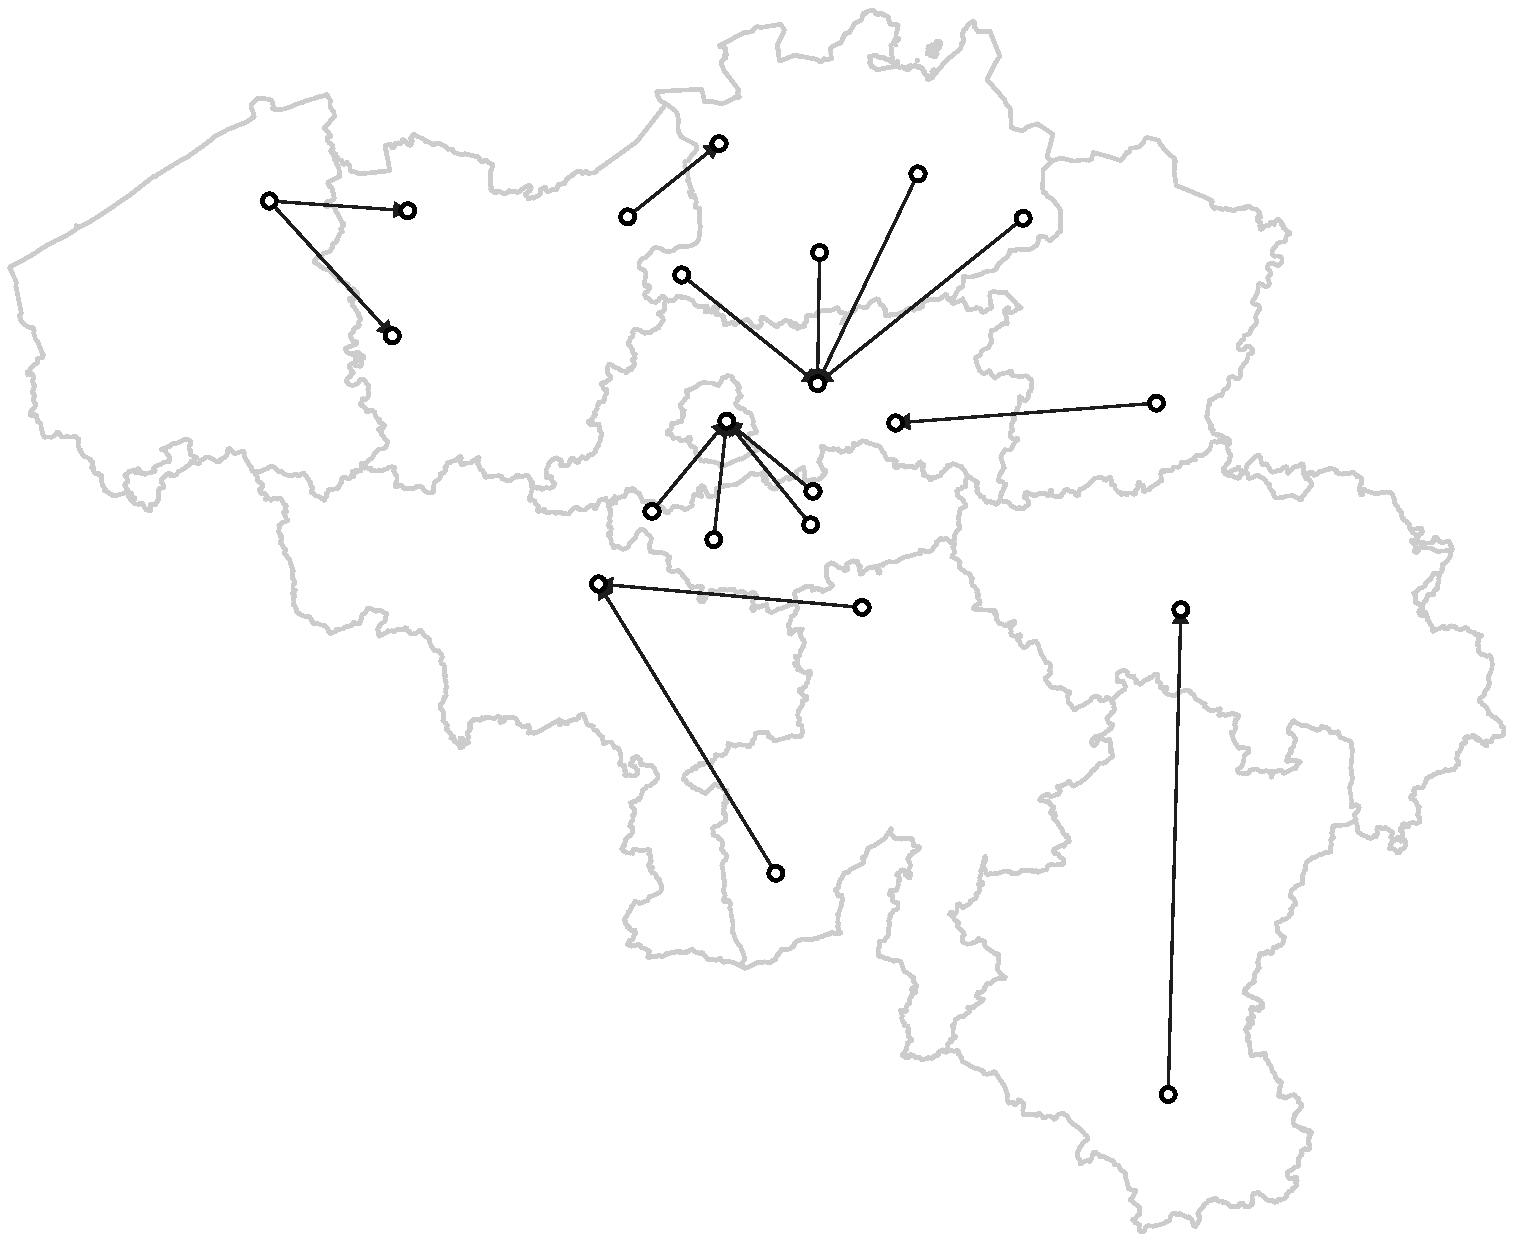
\includegraphics[width=4cm]{method-a.pdf}\\
    \subcaption{} % 4 words max
    \label{fig:method-a}
  \end{subfigure}%
  \begin{subfigure}{.2375\textwidth}
    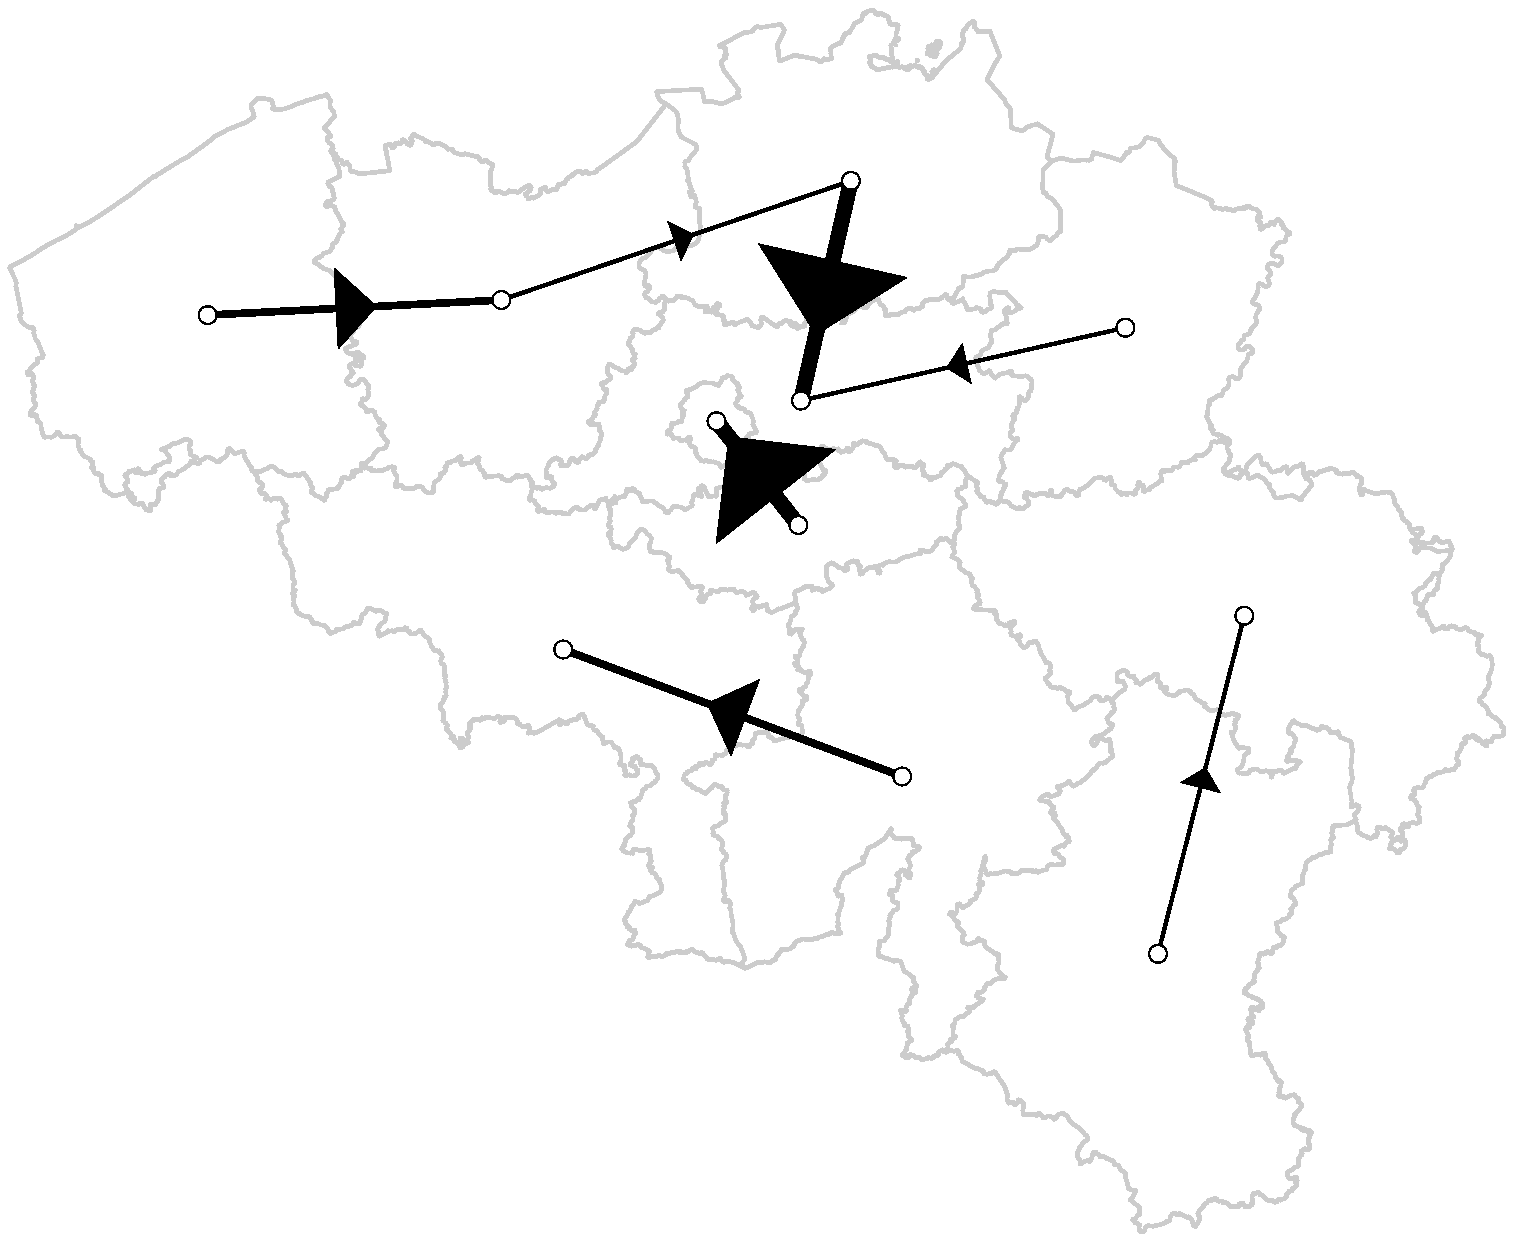
\includegraphics[width=4cm]{method-b.pdf}\\
    \subcaption{} % 4words max
    \label{fig:method-b}
  \end{subfigure}%
  \vspace{5.0pt}% To create a bit of vertical space between the 2 figure captions
  \caption{Spatial aggregation based on provincial administrative boundaries diagrammatically represented. (a) Individual data records are depicted geographically with arrows connecting origins to their respective destinations. (b) The result of aggregation is a set of weighted connections between provinces.}
  \label{fig:method-ab}
\end{figure}

Next, the data is aggregated so that province level flow patterns are emphasized.
\cref{fig:method-ab} provides a diagrammatic representation of spatial aggregation on the basis of provincial administrative boundaries.
To compare the volume of flow between rural provincial areas and urbanized zones, train stations in major cities were aggregated into seperate groups. 
Simiarly, stations located outside of Belgium were aggregated to distinct group. 
A diagrammatic breakdown is depicted in \cref{fig:method-c} where color and shape is used to demarcate each group.
The following types of flows are observable from the outcome of aggregation:

\begin{itemize}
  \item Travel from any provincial station to a major city.
  \item Travel between any two major cities.
  \item Travel between any two provincial stations.
  \item Travel between any international station to a major city.
  \item Travel between any international station to a provincial station.
\end{itemize}

\subsection{Visualization}\label{sec:vis}
%Flow visualizations are commonly employed to facilitate the comparison of aggregated movement. 
The chord diagram is a visualization technique based on the node-link metaphor that arranges nodes along the circumference of a circle \cite{krzywinski2009circos}. 
Each node is represented by an arc where its length is proportional to the total volume of incoming and outgoing flows. 
Chords or curved line segments are drawn to connect nodes. 
The width at the head or tail of each chord indicates the amount of movement relative frequency of movement from a certain location to another.
In our implementation of the chord diagram, nodes are colour coded to indicate individual provinces and the major cities located within their administrative boundaries. 
Interactive filtering is introduced to simplify the visualization and details are provided in pop-up dialogue when upon mouse-over.

\section{Results}
\label{sec:results}

In this chapter, we report on the results of studying visualizations with experts of \emph{Trein Tram Bus}\footnote{\url{http://treintrambus.be}}, a not for profit passenger federation.

\subsection{Time Based Analysis}
\begin{figure}[h]
\centering
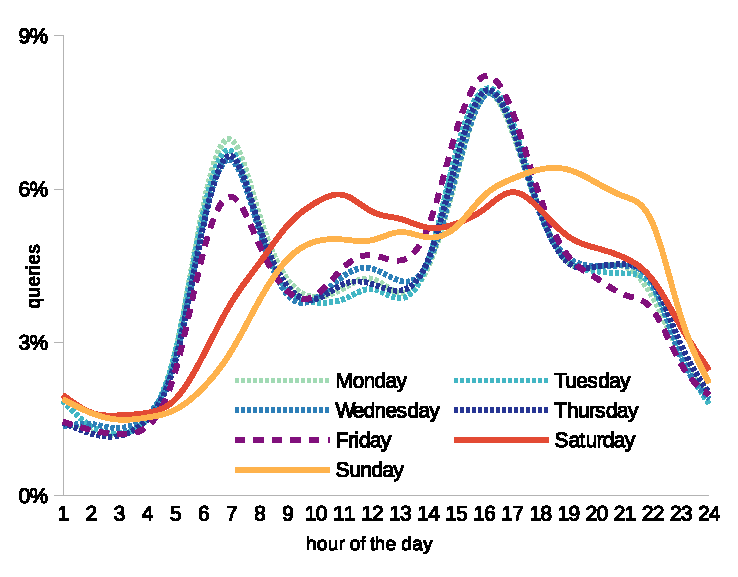
\includegraphics[width=8.6cm]{avg-all}
\caption{Distribution of iRail route planning API queries on average per day of the week between October 2012 and December 2015}
\label{fig:average}
\end{figure}

\begin{figure}[h]
\centering
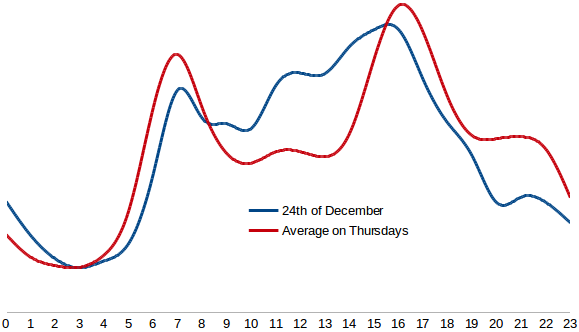
\includegraphics[width=8.6cm]{dec24}
\caption{Comparison of route planning queries on December 24th (Christmass Eve) 2015 with the average on a Thursday between October 2012 and December 2015. The illustration shows that people started going home earlier than usual.}
\label{fig:dec24}
\end{figure}

Results from the analysis of this dataset reveal trends in route planning queries that may provide insights into rail travel demand. 
First, the daily and hourly distribution of queries appear to correspond with known commuting patterns. 
\cref{fig:average} depicts a break down of the queries that occur, on average, on an hourly basis for each day of the week.
Several trends can be observed in this chart. 
Morning and evening peak periods in particular, are clearly distinguishable.
At noon, a small dent is noticable, which may be attributed to part time workers and meetings on location after or before noon.
Peak hours on weekdays are also distinctively different from those of weekends.
Similarly, the frequency of queries during the evening peak period on Fridays appear to be substantially higher than those that occur between Monday and Thursday.
The discrepancy maybe explained by students that travel home from their student homes over the weekends. 
The absence of a clear peak on Saturdays can be attributed to lack of journeys to work queries while the evening peak on Sundays may emerge from students returning to college accommodations.


Moreover, the distribution of queries on public holidays is observed to deviate from that of an average day. 
\cref{fig:dec24} provides a breakdown of queries per hour on Christmas eve, December 24th 2015, in comparison to an average Thursday of the same year. 
As illustrated, the evening peak on Christmas eve occurs earlier than that of an average Thursday. 
%For these reasons, we believe that route planning query data maybe a viable source of information for flow analysis.%\todo{where people are heading between certain time intervals?}

\subsection{Structure of Flows in Belgium}

The chord diagrams shown in \cref{fig:mornings} depict the aggregated number of queries made between any two stations on weekdays (see \cref{fig:weekdays_morning}) and weekends (see \cref{fig:weekends_morning}) respectively. 
An interactive version of this visualization can be viewed at \url{http://rxd.architectuur.kuleuven.be/irail/weekdays.html} and \url{http://rxd.architectuur.kuleuven.be/irail/weekends.html}. 
Visualizing our dataset in this manner reveals the complexity of flows on the Belgian rail system and the significance of cities in daily travel.
%We can observe that Brussels, Antwerp, Ghent and Leuven are the dominant destinations.
%Turning our attention to weekday travel, we can observe that Antwerp, Brussels and Ghent are the dominant destinations.
%The reverse occurs in the evening when trips are made towards provincial stations.
Brussels City stands out as the most distinctive visual element in both figures, indicating its function as the principal centre of rail activity (see \cref{fig:mornings}a).
On a regional level, its function as a centre appears to be more distinctive for the Walloon region than Flanders.
With exception to Liège city (see \cref{fig:mornings}e), queries from the Walloon region are generally made from provincial stations towards Brussels instead of major cities within their administrative boundaries. 
Queries from Flanders, on the hand, tend to be distributed among four major cities otherwise known as the Flemish Diamond, a network of metropolitan areas in Belgium comprised of Brussels, Antwerp (see \cref{fig:mornings}b), Ghent (see \cref{fig:mornings}c) and Leuven (see \cref{fig:mornings}d). 
These insights indicate that the structure of flows in Flanders appear to follow a polycentric pattern while that of the Walloon region is relatively monocentric, with Brussels city as a major centre.
The difference between both regions appear to correspond with existing measures of population density and degree of urbanisation, providing valuable insight as well as alternative perspectives into the function of cities in rural and urban settings.

\begin{figure*}
  \centering
  \begin{subfigure}{1\textwidth}
    \centering
    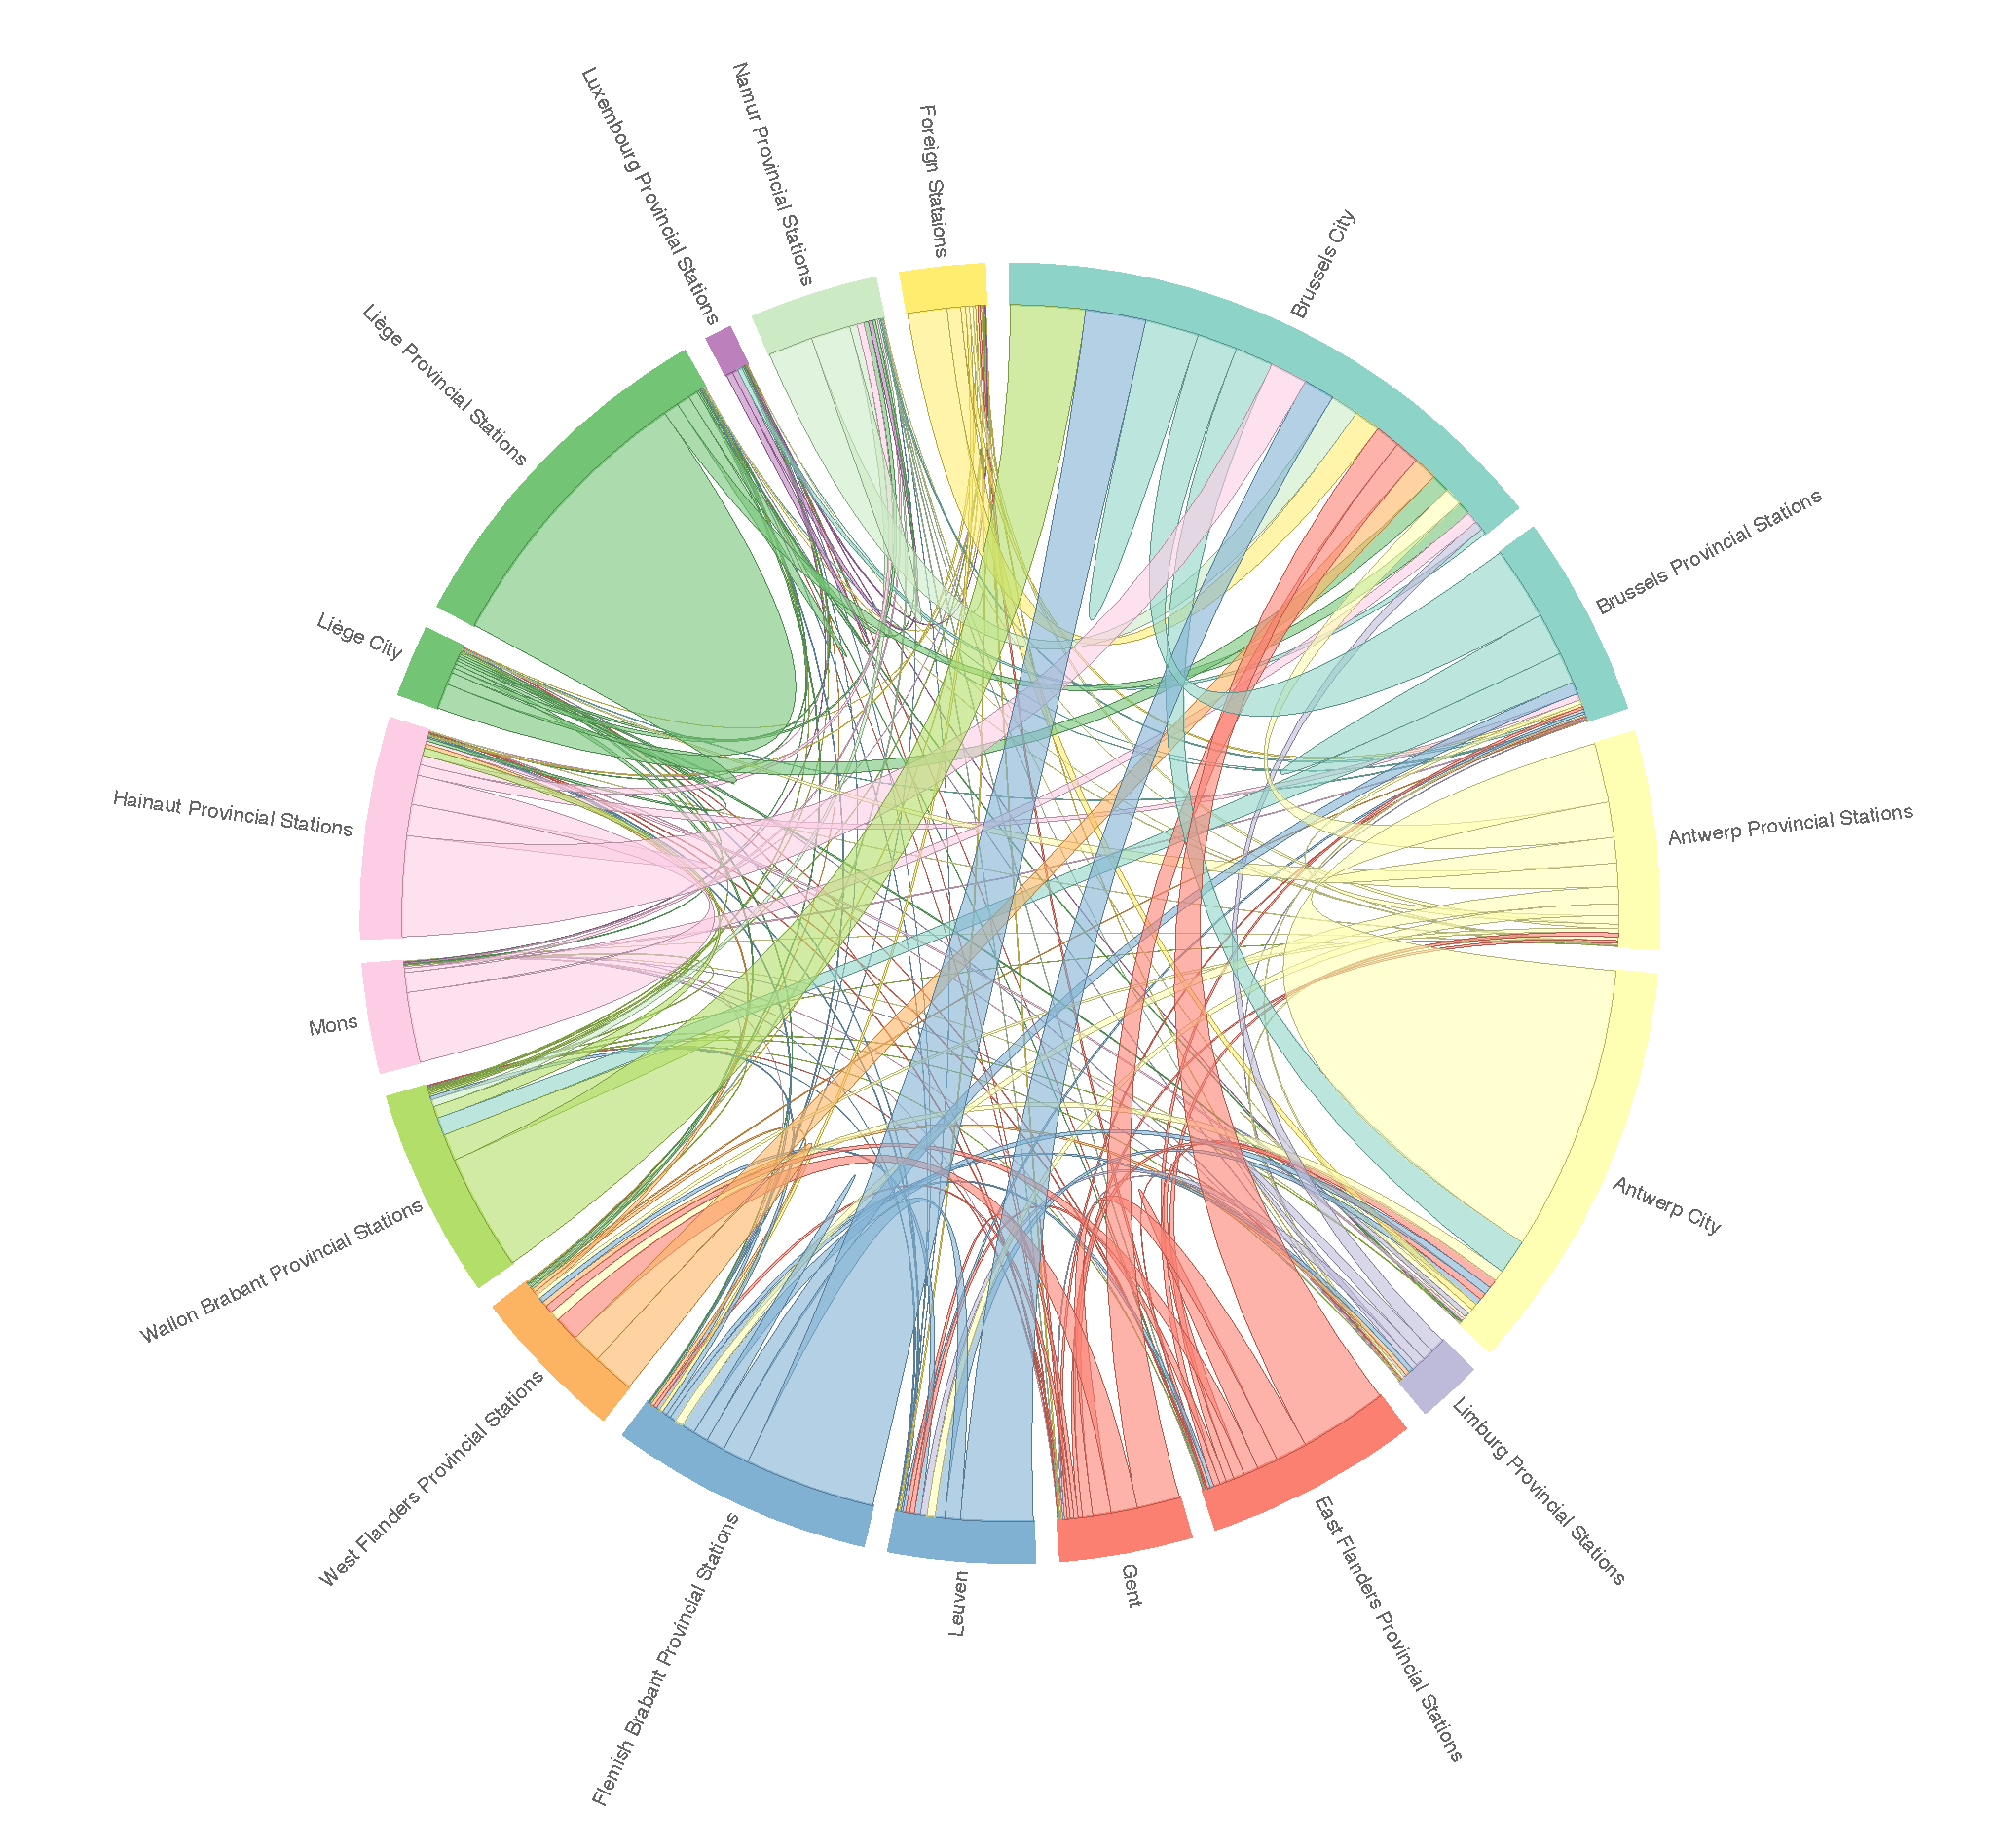
\includegraphics[width=13cm]{weekdays_morning.pdf}\\
    \subcaption{Weekdays} % 4 words max
    \label{fig:weekdays_morning}
  \end{subfigure}
  \begin{subfigure}{1\textwidth}
    \centering
    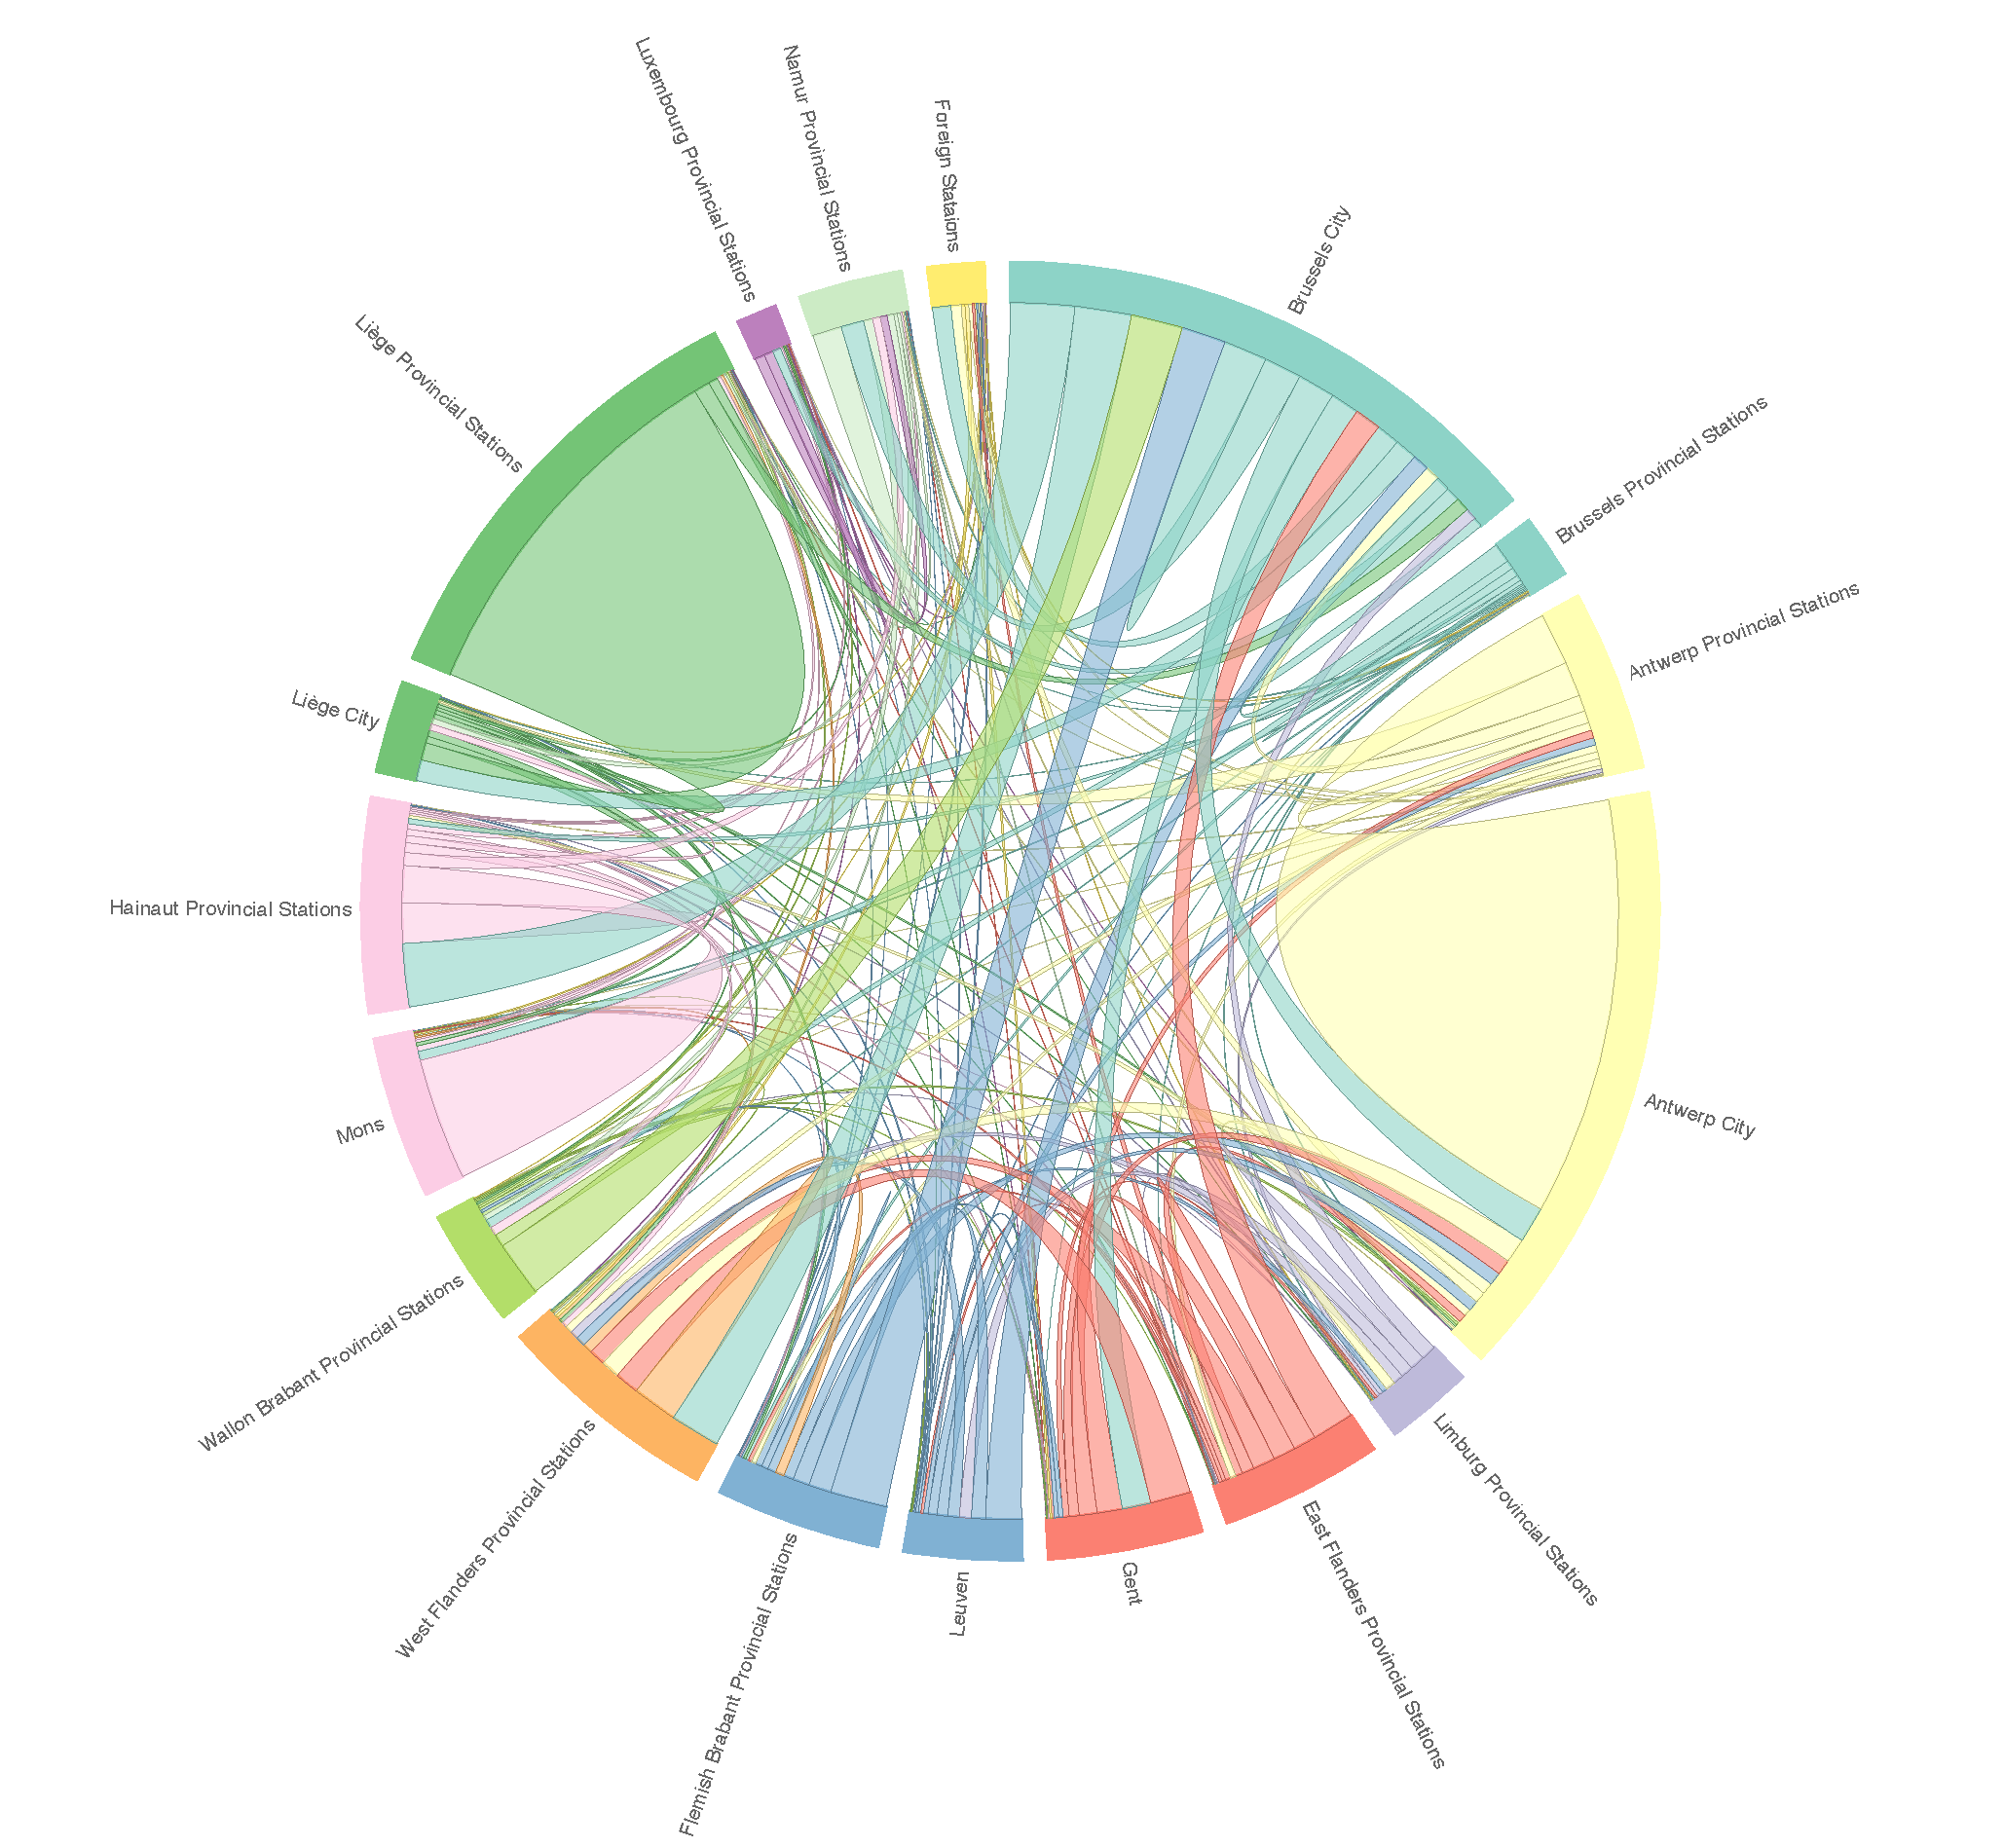
\includegraphics[width=13cm]{weekends_morning.pdf}\\
    \subcaption{Weekends} % 4words max
    \label{fig:weekends_morning}
  \end{subfigure}
  %\vspace{5.0pt}% To create a bit of vertical space between the 2 figure captions
  \caption{Comparison of morning rush hour travel flows on weekdays and weekends.}
  \label{fig:mornings}
\end{figure*}

\begin{figure*}[t]
\centering
\begin{tabular}{ccc}
  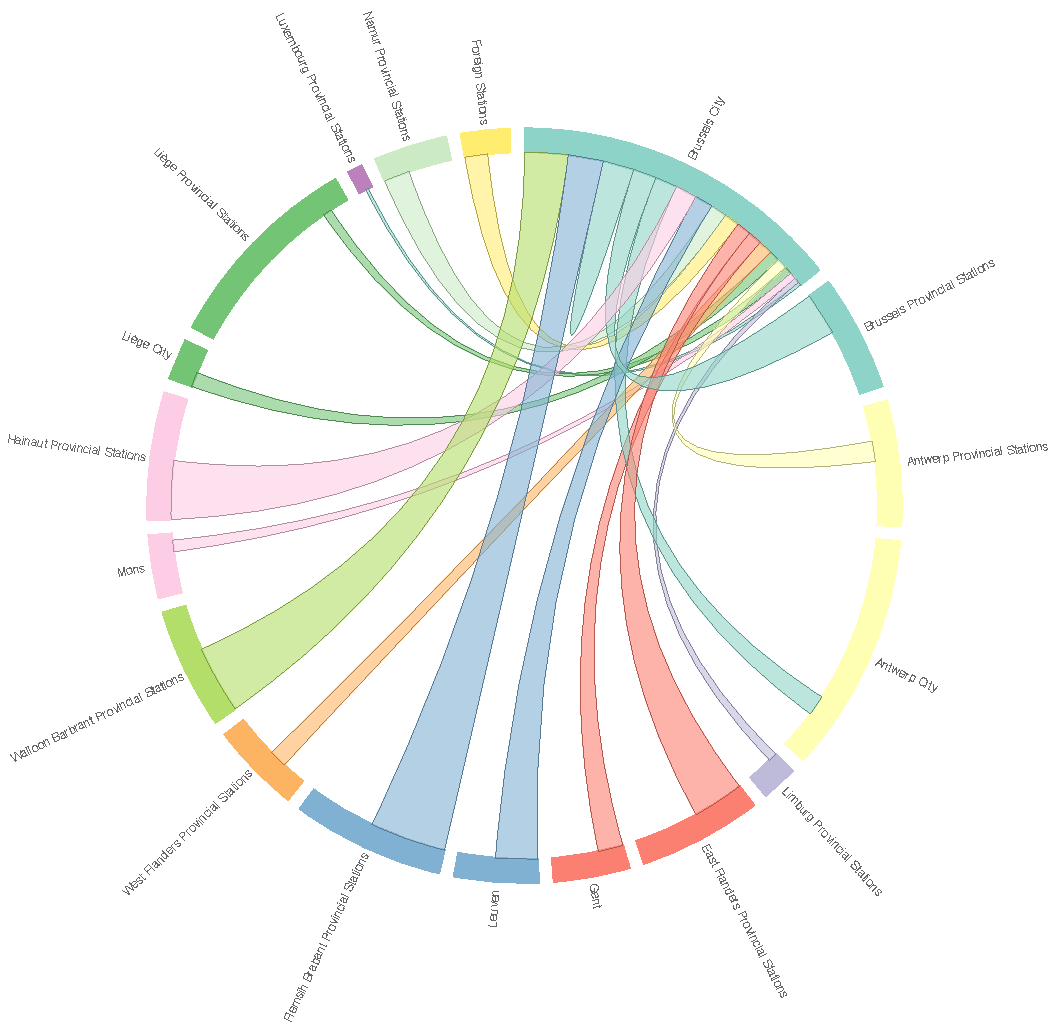
\includegraphics[width=.33\textwidth]{wd-brussels.pdf}& 
  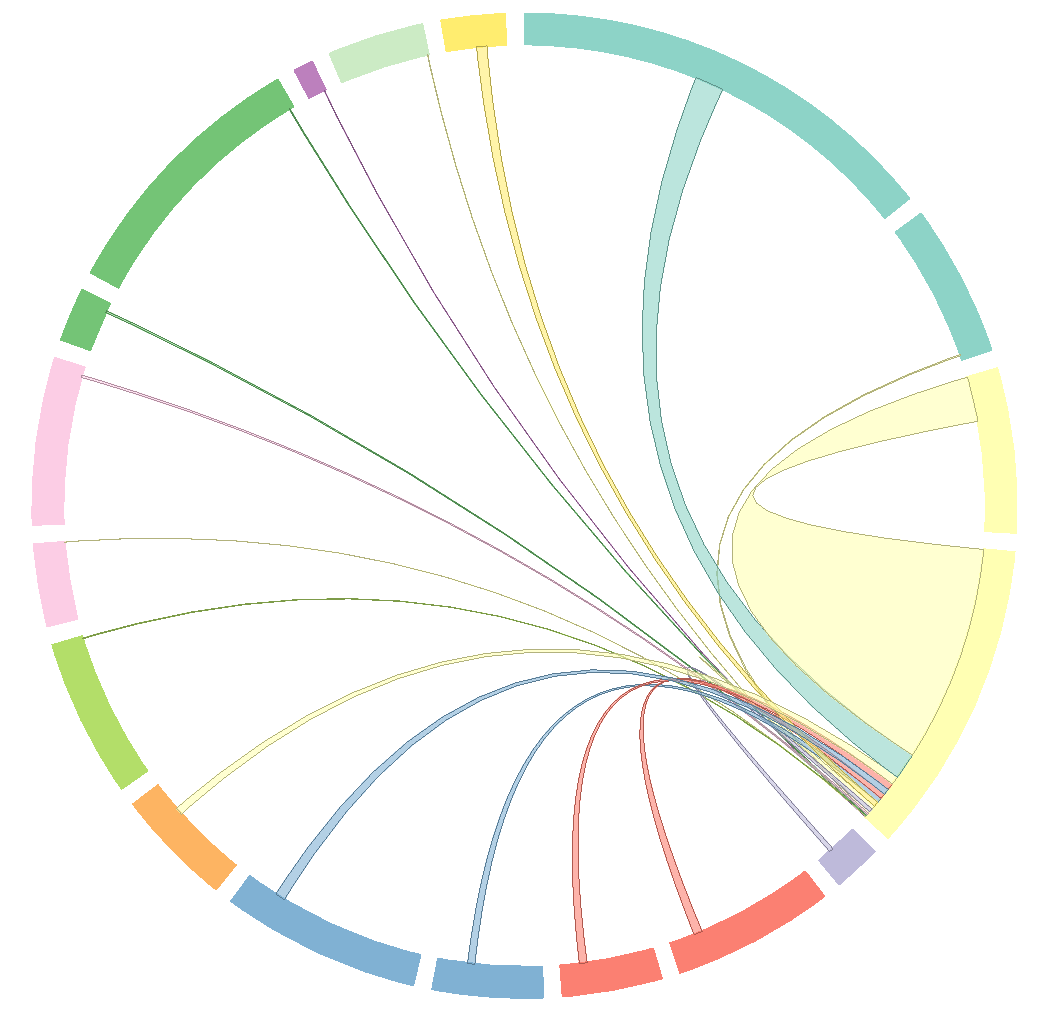
\includegraphics[width=.33\textwidth]{wd-antwerp.pdf}& 
  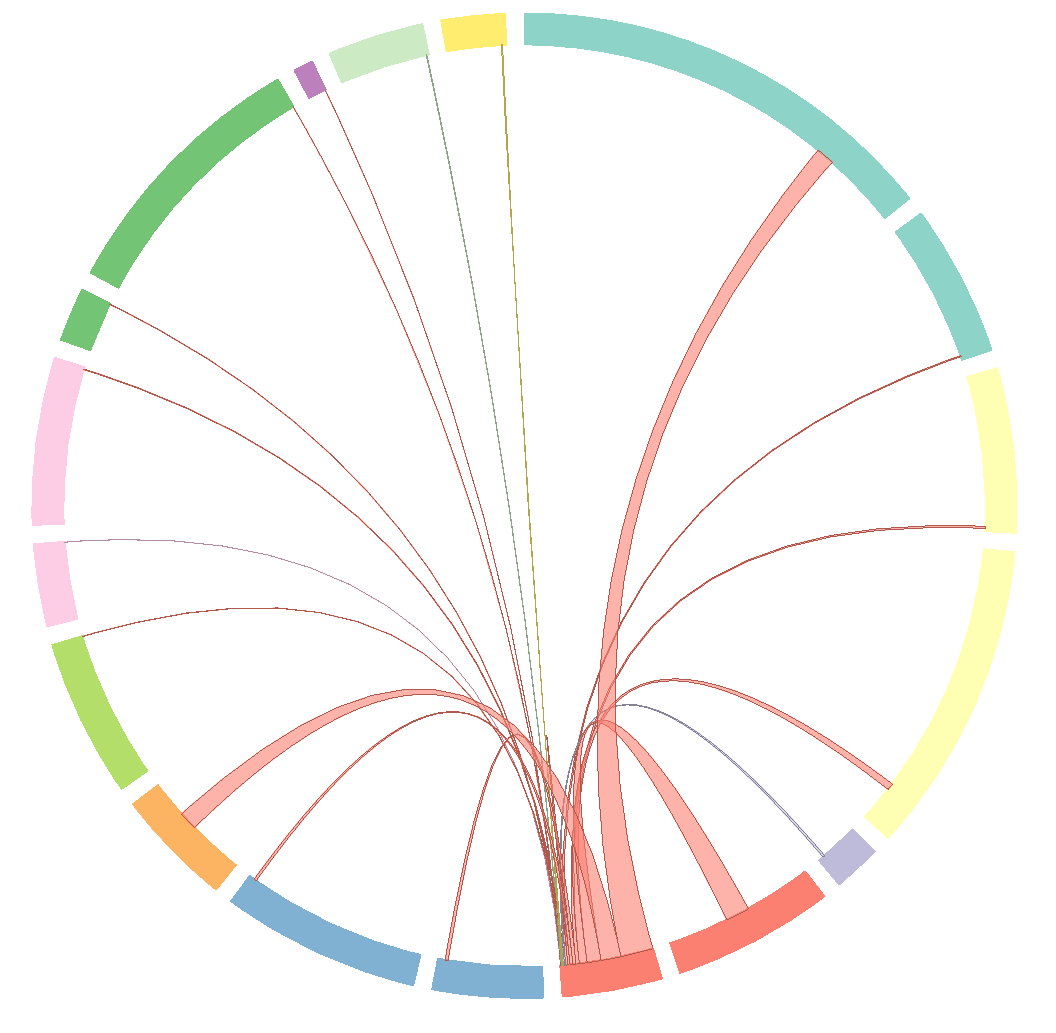
\includegraphics[width=.33\textwidth]{wd-gent.pdf}\\
  (a) Brussels City&(b) Antwerp City&(c) Ghent\\[6pt]
  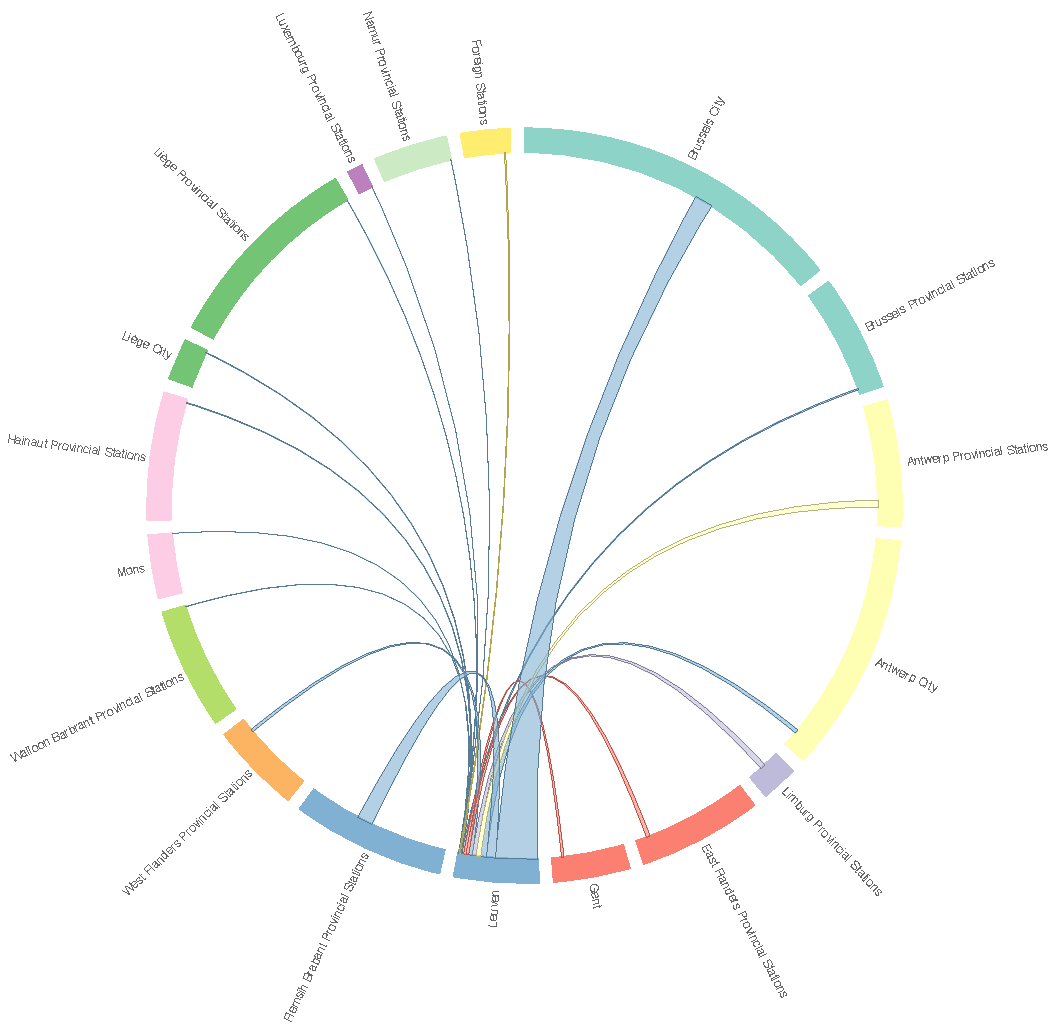
\includegraphics[width=.33\textwidth]{wd-leuven.pdf}& 
  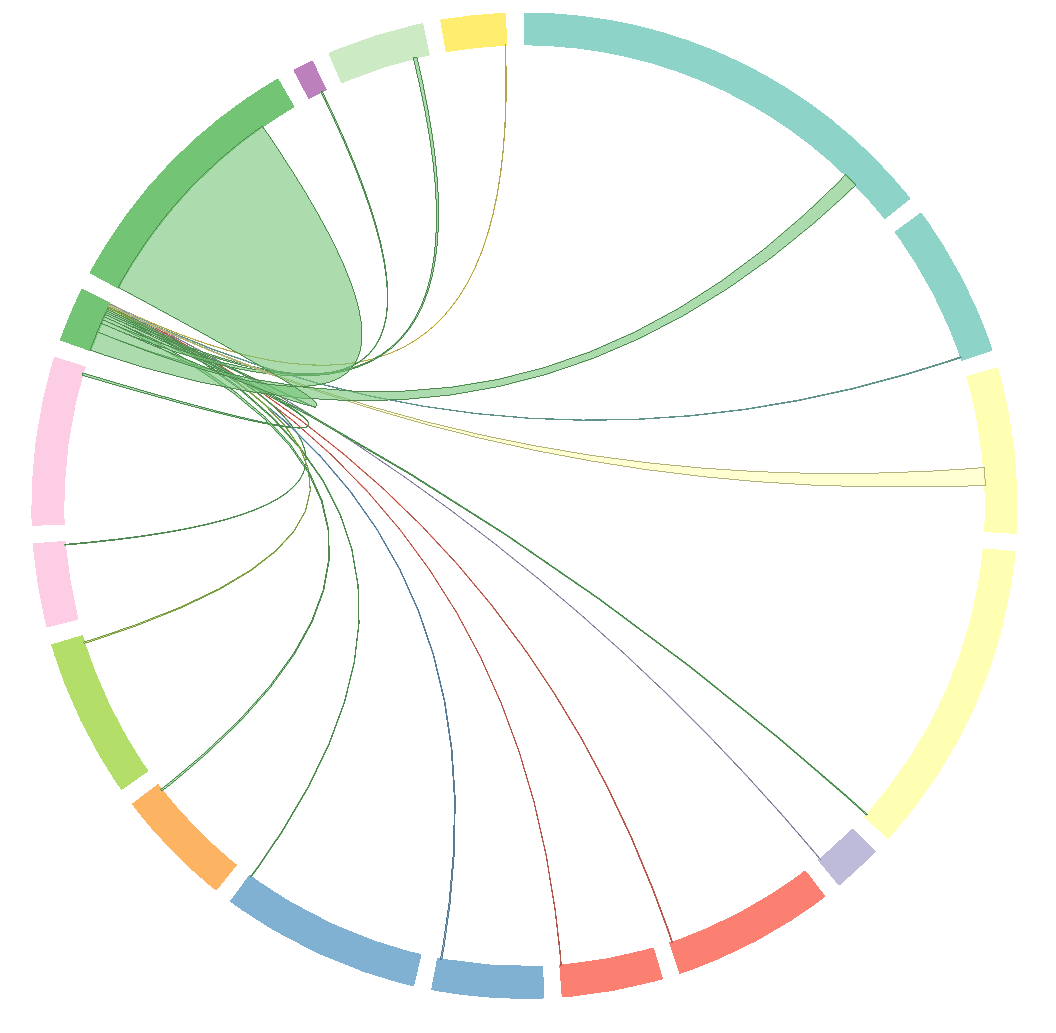
\includegraphics[width=.33\textwidth]{wd-liege.pdf}& 
  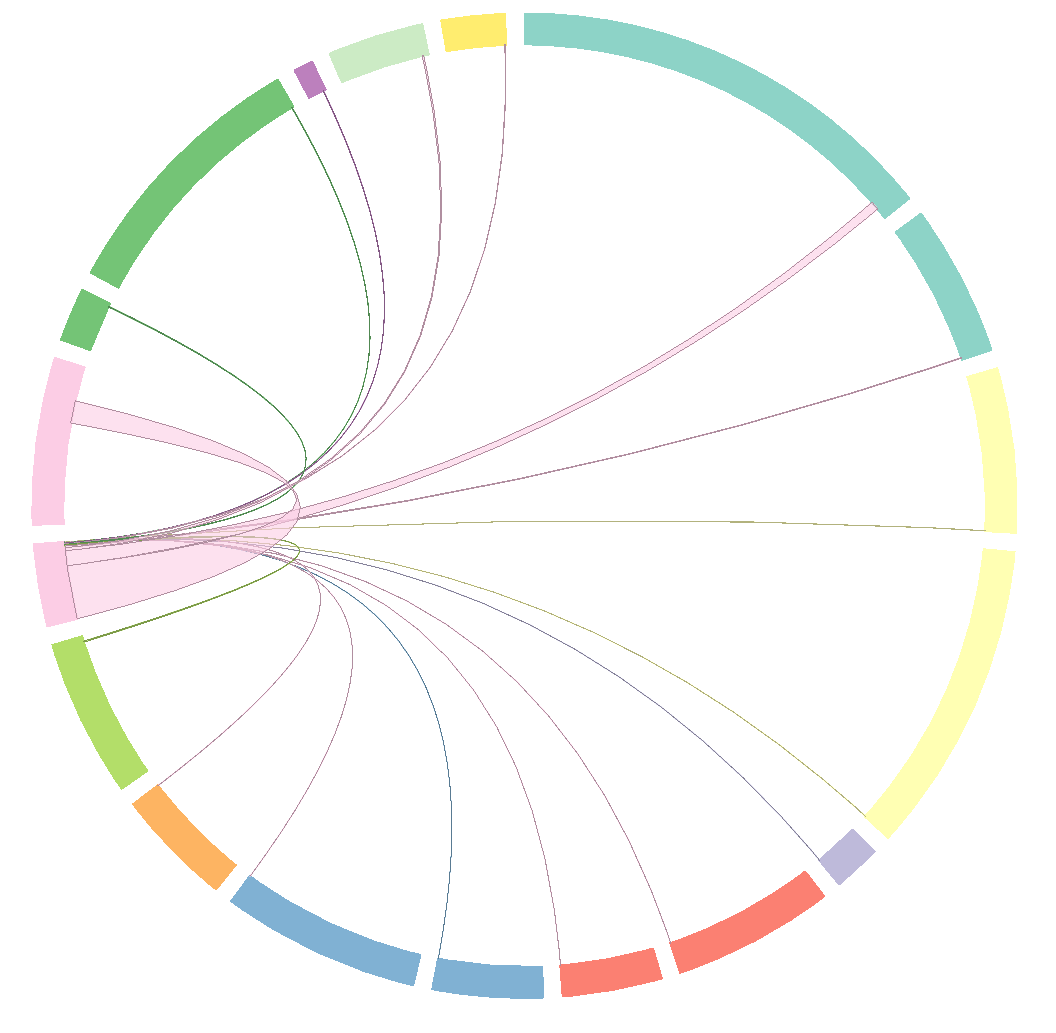
\includegraphics[width=.33\textwidth]{wd-mons.pdf}\\ 
  (d) Leuven&(e) Liège City&(f) Mons\\
\end{tabular}
\vspace{5.0pt}% To create a bit of vertical space between the 2 figure captions
\caption{Comparison of morning rush hour travel flows on weekdays originating from or destined for six major cities in Belgium.}
\label{fig:cities}
\end{figure*}


\subsection{Counter Intuitive Results}

There are several inconsistent patterns in the data that do not correspond with an existing understanding of flows in Belgium.
In particular, the large number of trips made between Antwerp city and other stations within the province of Antwerp in the morning, is not observable in other major cities in Flanders.
Further investigation led to the identification of an isolated connection originating from Antwerp city towards a suburb, suggesting anomalous usage of the iRail API that were not flagged as bots or a high concentration people who utilise route planning applications on a regular basis.
Alternatively the large number of trips may have originated from users who repeatedly request for updates on delayed trains or from a concentration of people who utilise route planning applications on a regular basis.
Accordingly, the reverse is identified in Liège where an unusually large connection originating from a suburb towards Liège city.
This prompted speculation, as well as discussions, on how such outliers should be treated or what may have led to their existence.
As with any form of analysis based on appropriation of data, we acknowledge that more work is required to identify caveats and understand the validity of the findings presented.

\section{Publishing transport data}
\label{sec:publishing}

The expressiveness of a server affects the way logs can be gathered~\cite{usewod2015}.
We have shown in previous sections that the query logs of a \emph{highly expressive server}, such as the iRail API, are interesting: each request contains an entire query which can be interpreted as a travel intention.
The possibility that two requests are exactly the same is low, as there are many URLs which can be requested.
Nevertheless, we cannot fully guarantee that each HTTP GET request to the server will trigger a log entry, due to caching mechanisms on the Web~\cite{fielding}, which might lead to a false representation.

%intermodality, features and availability
Hosting a route planning API as the only way to publish transport data comes with three identified limitations, as the server will need to handle the requests from different use cases with different needs:
\begin{enumerate}
  \item When an application developer would like a \emph{new feature}, such as taking wheelchair accessibility information into account, the feature would have to be implemented on the server of the data publisher.
  \item Keeping the server \emph{highly available} is costly, as any question can be asked by anyone for any purpose.
  \item Federated querying, which would allow for \emph{intermodal} route planning for route planning APIs, is inexistent up to date.
\end{enumerate}

% GTFS
In order to overcome these limitations, the General Transit Feed Specification (GTFS)\footnote{\url{https://developers.google.com/transit/gtfs/reference}} can be used. 
GTFS is a compressed ZIP-file containing a couple of CSV files, describing the rules for when a public transit vehicle will pass by on a certain location.
It is supported among all current open-source route planning software systems and it is used in products/apps such as \emph{CityMapper}, \emph{Ally}, \emph{Navitia.io}, \emph{Google Maps} and \emph{Bing Maps}.
%Persistence of the identifiers used within these datasets, is not a requirement, neither is it an ambition of the format\footnote{\url{https://groups.google.com/forum/#!msg/gtfs-changes/Z8Mf31MaZms/8Hc9F4psAQAJ}}.
%The goal of the format is to  an exchange format which specific software packages can use to transform it into their format of choice.
It succesfully enabled reuse for intermodal travel, engineers can rely on the data dumps even if the servers of the transit agency are offline and there is no limitation to the features that can be implemented.
The public transit agency however has no access any longer to an indication of travel demand.

In \cref{fig:LDFAxis2} we illustrate these two options as two extremes, with other options that are yet to be discovered.
When a server only allows to set e.g., a departure station and a departure time, then the server cannot log the arrival station, yet the client is still able to plan a route by executing the algorithm on the client-side~\cite{lc}.
We would be able to fully rely on the query logs if the expressivity would be maximal (extreme right) and caching would be turned off. 
Turning off caching may work in a private setting where you know how much and what kind of queries you can expect, yet on the open Web, caching helps decrease load on servers at peak moments.

%label: fig:LDFAxis2

% Linked Data Fragments axis
\begin{figure}[t]
  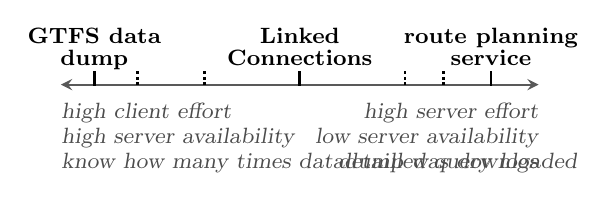
\begin{tikzpicture}[
    x=.005\textwidth,
    y=.1cm,
    axis/.style={
      line width=.8pt,
      stealth-stealth,
      color=black!65,
    },
    axislabel/.style={
      inner sep=0,
      font=\slshape\fontsize{8}{9}\selectfont,
      color=black!70,
    },
    tick/.style={
      line width=1pt,
    },
    ticklabel/.style={
      anchor=south,
      inner sep=0,
      align=center,
      font=\bfseries\fontsize{8}{8}\selectfont,
      text depth=0pt,
    },
  ]
    \newcommand\tick[2]{%
      \draw[tick] (#1, 1.7) -- (#1, -.4pt);
      \node[ticklabel] at (#1, 2.4) {#2};
    }
    \newcommand\vaguetick[1]{%
      \draw[tick,densely dotted] (#1, 1.7) -- (#1, -.4pt);
    }

    \draw[axis] (-100, 0) -- (0, 0);
    \node[axislabel,align=left,anchor=north west] at (-100, -2.3)
    {
%      generic requests\\
      high client effort\\
      high server availability\\
      know how many times datadump was downloaded
    };
    \node[axislabel,align=right,anchor=north east] at (0, -2.3)
    {
%      specific requests\\
      high server effort\\
      low server availability\\
      detailled query logs
    };

    \tick{-93}{GTFS data\\dump}
    \tick{-10}{route planning\\service}
    \tick{-50}{Linked\\Connections}

    \vaguetick{-84}    \vaguetick{-70}
    \vaguetick{-10}
    \vaguetick{-28}
    \vaguetick{-20}

   %\node[align=center,font=\fontsize{8}{9}\selectfont\bfseries] at (0, -8.3)
   %   {various types of\\Linked Data Fragments};
  \end{tikzpicture}
  \caption{This axis extends \cref{fig:LDFAxis1} with Linked Connections: a different choice of trade-offs for route planning advice over the Web.
  }
  \label{fig:LDFAxis2}
\end{figure}

\section{Conclusion and future work}
\label{sec:conclusion}

Firstly, we studied query logs to find travel patterns in Belgium.
We conclude that this is up to now, the best representation of travel flows over the Belgian railway network.%, as no alternatives are available.
We studied data which represent a maximum of 1.66\% of the passengers.
By visualizing the average distribution of requests on workdays and Saturday and Sunday, we were able to recognize the patterns we would expect: a.o. a morning and evening peak on workdays and a bigger evening peak on Friday and Sunday.
More interestingly, we were able to see that the evening peak on Christmass Eve, Thursday the 24th of December 2015, started earlier than average on Thursdays.
Visualizing our dataset using the origin and destination reveals the complexity of movement on the Belgian rail system and the significance of cities in weekday travel.
Furthermore, we found evidence that Flanders is polycentric, while Walloon traffic is monocentric.

Secondly, we also concluded that there are obvious caveats associated with the use of such data as proxy for actual statistical counts. 
We identified a couple of gaps:
\begin{enumerate}
  \item The data only captures an intention of an end-user: it is unsure whether the person actually took the train.
  \item Multiple user queries may be needed to cover a travel intention.
  \item Caching may mask peak hours, as many of the same requests in one minute is only stored in the logs once.
\end{enumerate}
Nevertheless, we published the query logs as open data at \url{http://api.irail.be/logs} for other scientists to continue to research possibilities with this dataset.
For instance, predicting trip congestion on the basis of this data, looks promising. %the iRail project is planning to use this data to predict trip congestion on the basis of this data.

Related work~\cite{verborgh2014lonesome} suggested to add additional metadata in the HTTP headers in order to track the user's intention.
While this is an interesting suggestion, it does not overcome the problem of caching.
In order to create a better representation of travel intentions, future work can gather logs by POST requests with the only purpose to gather analytics of travel intention.
This is a similar approach than what happens on the Web of Documents today with \emph{Piwik} or \emph{Google Analytics}.

% Fix spacing after References header (as line 1308 of sig-alternate.cls breaks it)
\let\oldsection\section
\renewcommand{\section}[2][1]{\oldsection{#1}\vspace{-3pt}}

\bibliographystyle{abbrv}
\bibliography{refs}
\end{document}
